% ============================================================
% TEMPLATE: Document với TikZ Figures
% Dùng cho: Bài tập, worksheet, tài liệu có nhiều hình
% ============================================================

\documentclass[12pt,a4paper]{article}

% === ENCODING & FONT ===
\usepackage[utf8]{inputenc}
\usepackage[T5]{fontenc}
\usepackage{times}

% === PAGE LAYOUT ===
\usepackage[margin=2cm]{geometry}

% === MATH ===
\usepackage{amsmath,amssymb}

% === TIKZ & LIBRARIES ===
\usepackage{tikz}
\usetikzlibrary{
    calc, arrows.meta, angles, quotes, positioning,
    patterns, shapes.geometric, decorations.pathmorphing
}

% === PGFPLOTS ===
\usepackage{pgfplots}
\pgfplotsset{compat=1.18}

% === CHEMFIG ===
\usepackage{chemfig}

% === CIRCUITIKZ ===
\usepackage{circuitikz}

% === FLOAT FIGURES ===
\usepackage{float}
\usepackage{caption}

% ============================================================
% CUSTOM STYLES
% ============================================================
\tikzset{
    point/.style={circle, fill, inner sep=1.5pt},
    main line/.style={thick},
    aux line/.style={thin, dashed, gray},
    vector/.style={-{Stealth[length=3mm]}, thick},
}

% ============================================================
% DOCUMENT
% ============================================================
\begin{document}

\begin{center}
    {\Large\bfseries BÀI TẬP HÌNH HỌC}\\[0.5em]
    {\normalsize Chủ đề: [Tên chủ đề]}
\end{center}

\vspace{1em}

% ============================================================
% BÀI TẬP 1
% ============================================================
\textbf{Bài 1.} Cho tam giác $ABC$ vuông tại $A$. Kẻ đường cao $AH$. 
Chứng minh rằng $AH^2 = BH \cdot HC$.

\begin{center}
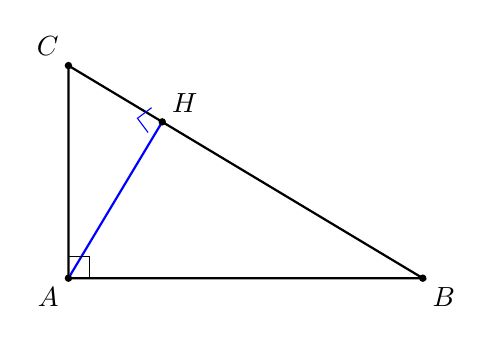
\begin{tikzpicture}[scale=0.9]
    % Định nghĩa đỉnh
    \coordinate (A) at (0,0);
    \coordinate (B) at (5,0);
    \coordinate (C) at (0,3);
    
    % Chân đường cao
    \coordinate (H) at ($(B)!(A)!(C)$);
    
    % Vẽ tam giác
    \draw[thick] (A) -- (B) -- (C) -- cycle;
    
    % Đường cao
    \draw[blue, thick] (A) -- (H);
    
    % Góc vuông tại A
    \draw (A) rectangle ++(0.3,0.3);
    
    % Góc vuông tại H
    \draw[blue] (H) ++(-0.15,0.2) -- ++(-0.2,-0.15) -- ++(0.15,-0.2);
    
    % Nhãn
    \node[below left] at (A) {$A$};
    \node[below right] at (B) {$B$};
    \node[above left] at (C) {$C$};
    \node[above right] at (H) {$H$};
    
    % Đánh dấu điểm
    \foreach \p in {A,B,C,H} \fill (\p) circle (1.5pt);
\end{tikzpicture}
\end{center}

\vspace{1em}

% ============================================================
% BÀI TẬP 2
% ============================================================
\textbf{Bài 2.} Cho đường tròn $(O; R)$ và điểm $A$ nằm ngoài đường tròn. 
Từ $A$ kẻ tiếp tuyến $AT$ với đường tròn ($T$ là tiếp điểm).

\begin{center}
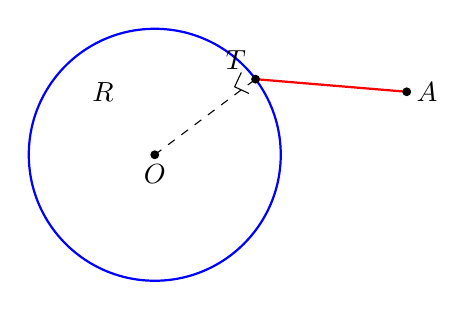
\begin{tikzpicture}[scale=0.8]
    % Đường tròn
    \coordinate (O) at (0,0);
    \def\R{2}
    \draw[thick, blue] (O) circle (\R);
    
    % Điểm A ngoài đường tròn
    \coordinate (A) at (4,1);
    
    % Điểm tiếp xúc T (tính toán)
    \coordinate (T) at (1.6, 1.2);
    
    % Tiếp tuyến AT
    \draw[red, thick] (A) -- (T);
    
    % Đường OT
    \draw[dashed] (O) -- (T);
    
    % Góc vuông tại T
    \draw (T) ++(155:0.25) -- ++(245:0.25) -- ++(335:0.25);
    
    % Nhãn
    \fill (O) circle (2pt);
    \fill (A) circle (2pt);
    \fill (T) circle (2pt);
    \node[below] at (O) {$O$};
    \node[right] at (A) {$A$};
    \node[above left] at (T) {$T$};
    \node[left] at (-0.5, 1) {$R$};
\end{tikzpicture}
\end{center}

\vspace{1em}

% ============================================================
% BÀI TẬP 3 - Đồ thị
% ============================================================
\textbf{Bài 3.} Vẽ đồ thị hàm số $y = x^2 - 2x - 3$ và tìm các giao điểm với trục $Ox$.

\begin{center}
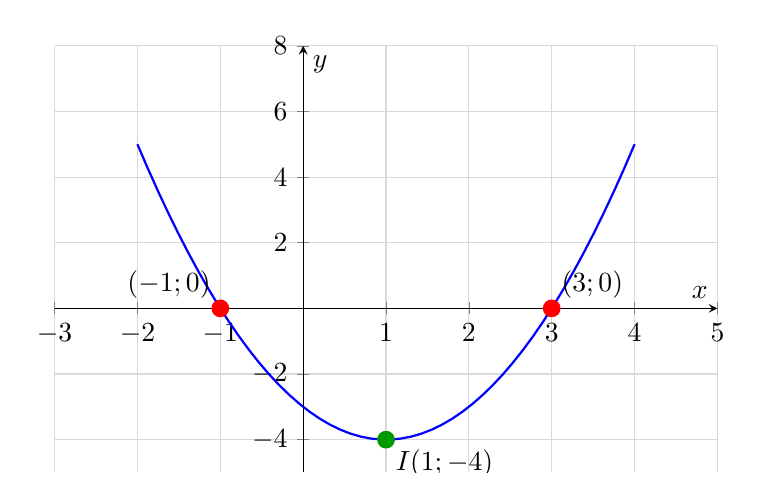
\begin{tikzpicture}
\begin{axis}[
    axis lines=middle,
    xlabel={$x$}, ylabel={$y$},
    xmin=-3, xmax=5,
    ymin=-5, ymax=8,
    grid=both,
    grid style={gray!30},
    width=10cm, height=7cm,
]
    % Parabol
    \addplot[blue, thick, domain=-2:4, samples=50] {x^2 - 2*x - 3};
    
    % Giao điểm với Ox
    \addplot[mark=*, only marks, red, mark size=3pt] coordinates {(-1,0) (3,0)};
    
    % Đỉnh
    \addplot[mark=*, only marks, green!60!black, mark size=3pt] coordinates {(1,-4)};
    
    \node[above left] at (axis cs:-1,0) {$(-1;0)$};
    \node[above right] at (axis cs:3,0) {$(3;0)$};
    \node[below right] at (axis cs:1,-4) {$I(1;-4)$};
\end{axis}
\end{tikzpicture}
\end{center}

\vspace{1em}

% ============================================================
% BÀI TẬP 4 - Hóa học
% ============================================================
\textbf{Bài 4.} Viết công thức cấu tạo của các chất sau:

a) Axit axetic (CH$_3$COOH):
\begin{center}
    \chemfig{H_3C-C(=[2]O)-O-H}
\end{center}

b) Etanol (C$_2$H$_5$OH):
\begin{center}
    \chemfig{H_3C-CH_2-OH}
\end{center}

c) Benzen (C$_6$H$_6$):
\begin{center}
    \chemfig{**6(------)}
\end{center}

% ============================================================
\end{document}
